\chapter{Projektkontext}

\section{Das Projekt Charigame}

Das Projekt Charigame entstand ursprünglich als interne Initiative der elancer-team GmbH mit dem Ziel eine digitale Spendenaktion zu ermöglichen.
Diese Idee des Projekts lässt sich auf eine durch die Agentur erstellte Weihnachtsaktion zurückführen, die auf der Website \texttt{https://hohoho.elancer-team.de/} implementiert wurde.
Bei der Spendenaktion hat die elancer-team GmbH die Spendensumme bereitgestellt und die Agenturkunden wurden eingeladen teilzunehmen und durch ihr engagement den Spendentopf zu erhöhen.
Diese Plattform ermöglichte es den Kunden der Agentur erstmals, über die gamifizierte Benutzeroberfläche Spenden zu erspielen und zu verteilen.
\\\\
Die positive Resonanz der Agenturkunden auf diesen gamifizierten Ansatz führte zu der Überlegung das Konzept weiterzuentwickeln.
Aufgrund der erfolgreichen Durchführung äußerte ein Kunde der Agentur den Wunsch, eine vergleichbare Spendenaktion für das eigene Unternehmen zu realisieren.

Diese erste kundenspezifische Umsetzung basierte auf einer abgewandelten Kopie der Weihnachts-Spendenaktion.
Die Anfrage stellte dann den Übergang von einem internen Projekt zu einem eigenständigen Dienstleistungsangebot dar.
Daraufhin wurde durch den Autor das Projekt Charigame als eigenständiges WordPress-Plugin realisiert.
Das daraus resultierende WordPress-Plugin befindet sich aktuell bei einem Kunden im produktiven Einsatz und bildet die Grundlage für die in dieser Arbeit dokumentierten technischen Analyse und Weiterentwicklung.
\\\\
\textbf{Funktionsweise von Charigame}
\\\\
Die Funktionsweise von Charigame lässt sich grob in 5 Schritte unterteilen, die in Abbildung~\ref{fig:charigame-funktion}: veranschaulicht sind:

%\begin{figure}[!ht]
%    \centerline{\includesvg[width=1\columnwidth]{images/firstPartyCookie.svg}}
%    \caption{Entstehungsprozess von First Party Cookies}
%\end{figure}
\begin{figure}[tbh]
    \centering
    \includesvg[width=0.66\textwidth]{images/funktionsweise_charigame}
    \caption{Funktionsweise Charigame (eigene Darstellung)}
    \label{fig:charigame-funktion}
\end{figure}
\newpage

\begin{enumerate}
    \item \textbf{Aufbau der Kampagne und Mailing}
    \\ Eine Spendenkampagne wird im Backend von Charigame angelegt.
    Anschließend werden Personendaten der Kunden in das System importiert.
    Das System versendet dann, basierend auf den Kampagneneinstellungen, automatisierte E-Mails mit dem Link zur Spendenaktion.
    \item \textbf{Kundeninteraktion und Spendenspiel}
    \\ Der Kunde öffnet den personalisierten Code in der E-Mail oder gibt den darin enthaltenen Code auf der Login-Page ein.
    Die in der Kampagne eingestellte Charigame-Landingpage wird angezeigt und der Kunde kann aktiv beim Spendenspiel teilnehmen.
    \item \textbf{Spielende und Spendenverteilung}
    \\ Nachdem das Spendenspiel seitens des Kunden absolviert wurde, kann dieser den erspielten Beitrag prozentual auf einen von bis zu drei verschiedenen Spendenempfängern verteilen.
    \item \textbf{Dankesseite}
    \\ Eine Dankesseite wird angezeigt und der Kunde kann nach Belieben erneut an dem Spiel teilnehmen, um seine Punktzahl zu verbessern.
    Ferner werden weitere Handlungsauforderungen in Form von CTAs ausgespielt, die den Kunden gezielt auf Bereiche des Unternehmens leiten können.
\end{enumerate}

\section{Deskriptiver Stand}
\subsection{Wordpress Front- und Backend}
Der deskriptive Stand von Charigame befindet sich in einem funktionsfähigen, jedoch technisch und konzeptionell ausbaufähigen Zustand.
Das WordPress-Plugin integriert sich in das CMS WordPress und erweitert den Funktionsumfang, um gamifizierte Spendenaktionen.
Bevor die Spendenaktion bereitsteht ist es notwendig, dass verschiedene Einstellungen getroffen.
Die notwendigen Einstellungen können über das WordPress-Backend Menü aufgerufen werden.
\\
Hierzu erzeugt ein Charigame Menüpunkt im WordPress Dashboard wie in Abbildung~\ref{fig:charigame-menu-legacy}: visualisiert.
In diesem Menü sind die wichtigsten Einstellmöglichkeiten als Menüpunkte definiert.
\begin{figure}[tbh]
    \centering
    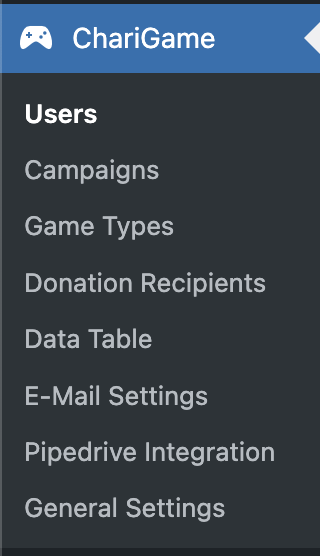
\includegraphics[width=0.2\textwidth]{images/legacy_charigame_wordpress_menu}
    \caption{Charigame Menü im WordPress Dashboard (eigene Darstellung)}
    \label{fig:charigame-menu-legacy}
\end{figure}

Die im Menü angezeigten Einstellungen und Informationen lassen sich in mehrere Kategorien gliedern.
Diese spiegeln den Aufbau der einzelnen Bausteine vom Projekt wider und werden nachfolgend erläutert.
\\\\
\textbf{General Settings}\\\\
Die General Settings enthalten grundlegende Angaben zum Unternehmen, das eine Spendenkampagne durchführt.
Neben rechtlichen Informationen wie dem Impressum und der AGBs können hier auch gestalterische Parameter wie Farben der Corporate Identity hinterlegt werden.
Die Backendansicht der Einstellungsseite ist in Abbildung~\ref{fig:charigame-general-settings-legacy} dargestellt.
\begin{figure}[H]
    \centering
    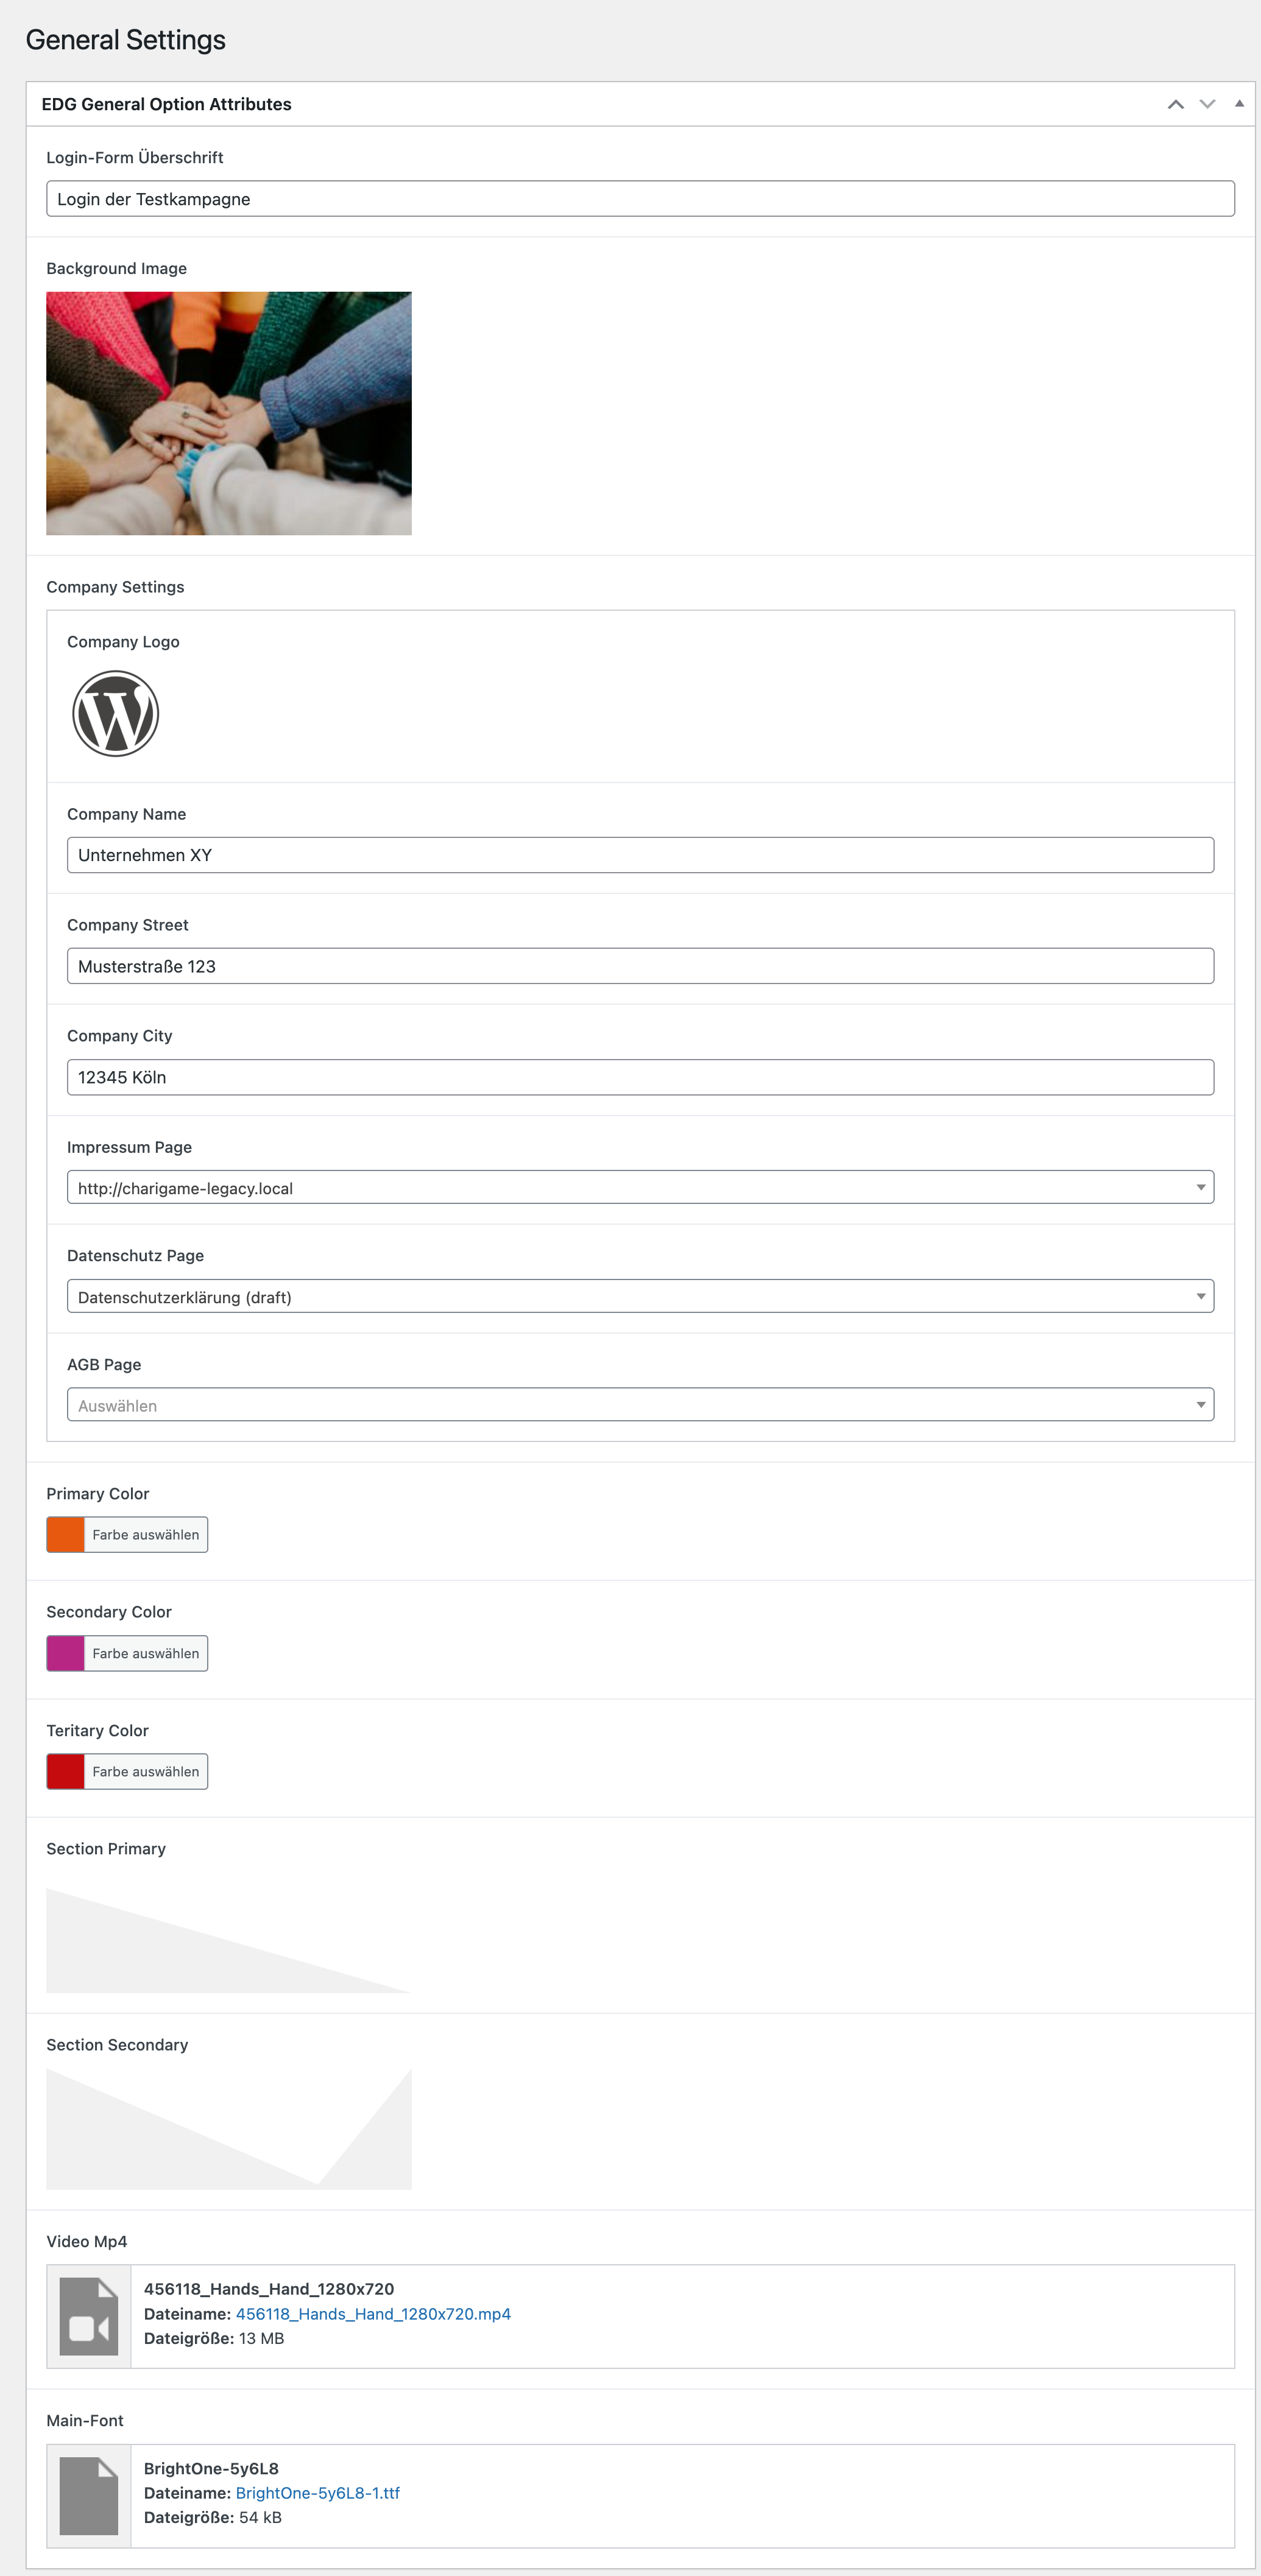
\includegraphics[width=0.7\textwidth]{images/legacy_general_settings}
    \caption{Screenshot aus dem WordPress-Backend (eigene Darstellung).\\
    Enthaltene Medien:\\Hintergrundbild © Aditya Romansa / Unsplash \cite{unsplash_romansa_babyhand},\\
    Logo © WordPress Foundation \cite{wordpresslogo}.}
    \label{fig:charigame-general-settings-legacy}
\end{figure}

Es können grundlegende Einstellungen konfiguriert werden, z.B.:
\begin{itemize}
\item Überschriften der Login-Form
\item Hintergrund- und Logo-Uploads
\item Farbschema (Primär, Sekundär, Teritär)
\end{itemize}
Eine vollständige Übersicht der Eingabefelder ist im Anhang zu finden (vgl. Tabelle~\ref{tab:eingabefelder_general_settings}).
\\\\
Die getroffenen Einstellungen bestimmen direkt das Erscheinungsbild der Login-Form im Frontend (vgl. Abbildung~\ref{fig:login-textkampagne}).

\begin{figure}[H]
    \centering
    
\includegraphics[width=0.8\textwidth]{images/legacy_login_testkampagne}
    \caption{Login-Form einer Charigame-Testkampagne im Frontend (eigene Darstellung)}
    \label{fig:login-textkampagne}
\end{figure}

\textbf{Donation Recipients}\\\\
Die Donation Recipients stellen die Empfänger der Spenden dar.
Für jede Kampagne müssen mindestens drei Empfänger angelegt werden.
Pro Empfänger werden ein Name, ein Bild sowie ein beschreibender Text hinterlegt (vgl. Tabelle~\ref{tab:eingabefelder_donation_recipients}).
Das vorab erstellen der Recipients ist im Verlauf der Einstellungen zwingend erforderlich, da sie in den Kampagneneinstellungen referenziert werden.
Die Backendansicht der Donation Recipients ist in Abbildung~\ref{fig:donation-recipients-settings-legacy} veranschaulicht.
\begin{figure}[H]
    \centering
    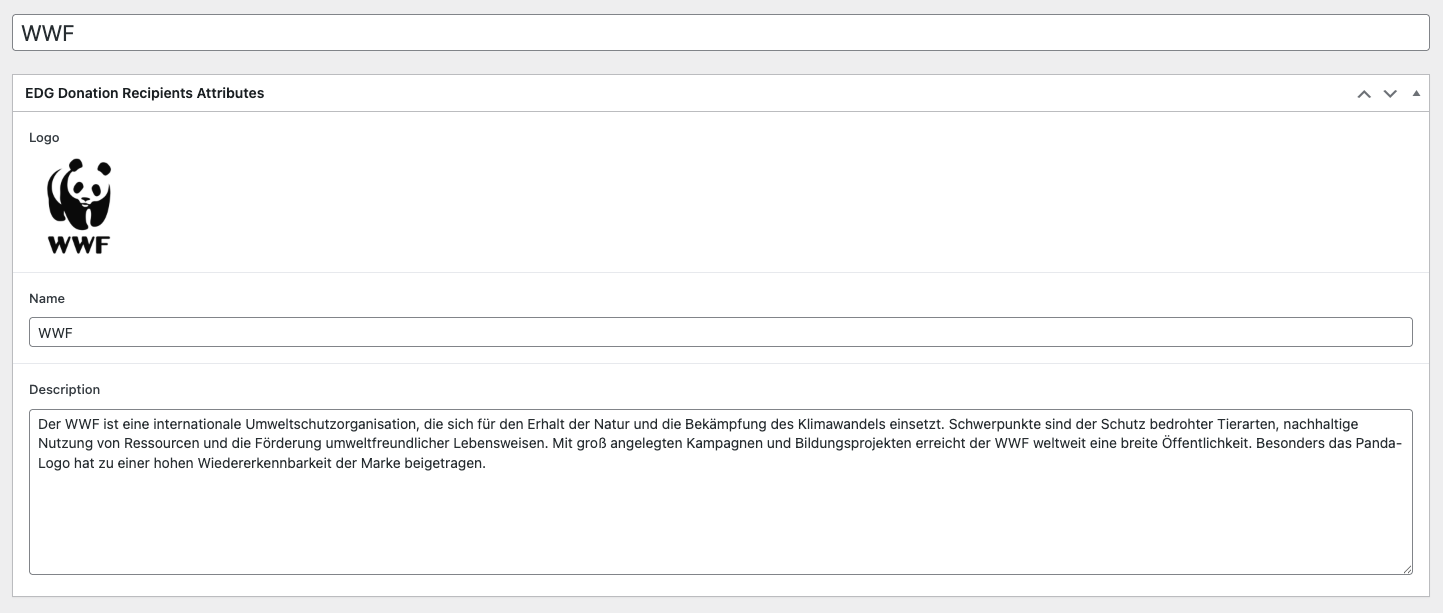
\includegraphics[width=1\textwidth]{images/legacy_donation_recipients_backend}
    \caption{Donation Recipients im WordPress Backend (eigene Darstellung)}
    \label{fig:donation-recipients-settings-legacy}
\end{figure}
Die im Backend gesetzten Einstellungen werden in folgender Form wie (vgl. Abbildung~\ref{fig:donation-recipients-frontend-legacy}) im Frontend dargestellt:
\begin{figure}[H]
    \centering
    
\includegraphics[width=1\textwidth]{images/legacy_donation_recipients_frontend}
    \caption{Donation Recipients im WordPress Frontend (eigene Darstellung)\\Enthaltene Logos © UNICEF, Deutsches Rotes Kreuz, WWF \cite{ngo_logos}}
    \label{fig:donation-recipients-frontend-legacy}
\end{figure}

\newpage
\textbf{Game Types}\\\\
Unter Game Types werden die verfügbaren Spieltypen definiert.
Jedes Spiel kann vom Unternehmen mit einer \glqq How-To-Play\grqq{}-Anleitung versehen werden.
Diese besteht aus einer Abfolge von Schritten, die jeweils mit einem Icon, einer Überschrift und einem erklärenden Text ergänzt werden können.
Im Detail können die verfügbaren Attributionen aus der Tabelle~\ref{tab:eingabefelder_game_types} entnommen werden.
Die Backendansicht der Game Types ist in Abbildung~\ref{fig:game-types-settings-legacy} ersichtlich.
\begin{figure}[H]
    \centering
    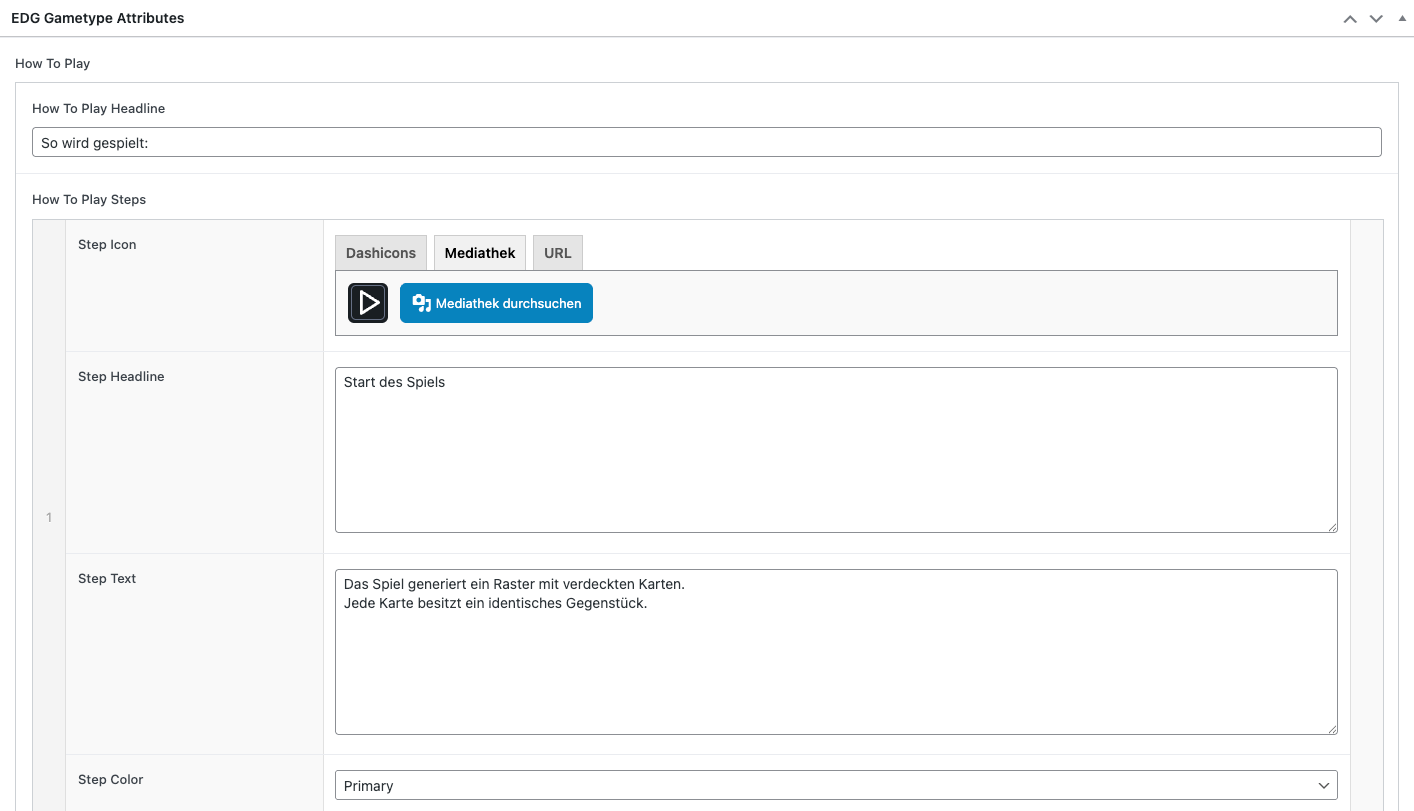
\includegraphics[width=1\textwidth]{images/legacy_game_types_backend}
    \caption{Game Types im WordPress Backend (eigene Darstellung)}
    \label{fig:game-types-settings-legacy}
\end{figure}
Wenn entsprechende Informationen eingepflegt sind erzeugt der Bereich der Game Types den folgenden Frontend View wie in Abbildung~\ref{fig:game-types-frontend-legacy} zu sehen:
\begin{figure}[H]
    \centering
    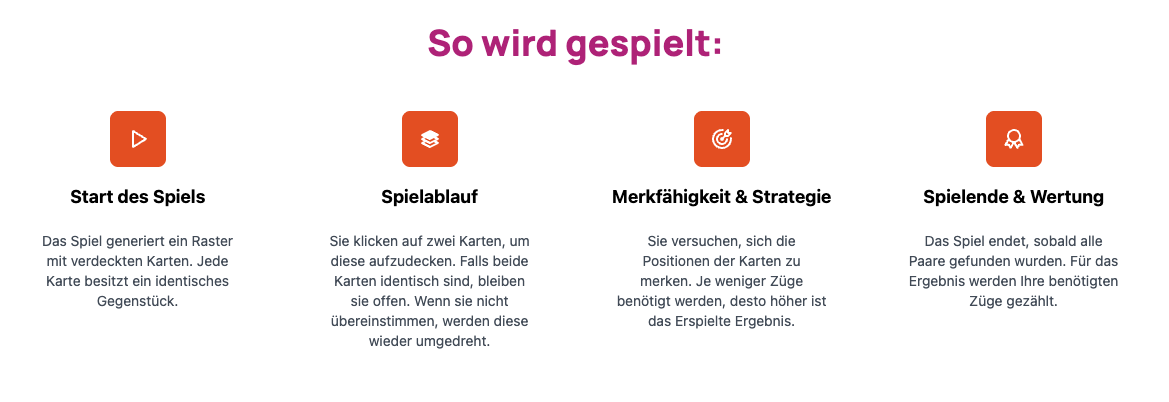
\includegraphics[width=1\textwidth]{images/legacy_game_types_frontend}
    \caption{Game Types im WordPress Frontend (eigene Darstellung)}
    \label{fig:game-types-frontend-legacy}
\end{figure}

\\\\
\textbf{Users \& Pipedrive Integration}\\\\
Die Menüpunkte Users und Pipedrive Integration dienen maßgeblich der Verwaltung im Backend und haben keine direkten Auswirkungen auf das Frontend.
Im Bereich der Users werden die Teilnehmer der Spendenkampagnen verwaltet und diesen können die folgenden Werte zugeordnet werden:
\begin{itemize}
    \item Vorname
    \item Nachname
    \item Geburtsdatum
    \item E-Mail-Adresse
    \item Flags: Imported, Email sent
\end{itemize}
Die genauen Werte und Eingabetypen können aus der Tabelle~\ref{tab:eingabefelder_users} entnommen werden.
Im WordPress Backend wird die User Sektion wie folgt Dargestellt (vgl. Abbildung~\ref{fig:users-backend-legacy})

\begin{figure}[H]
    \centering
    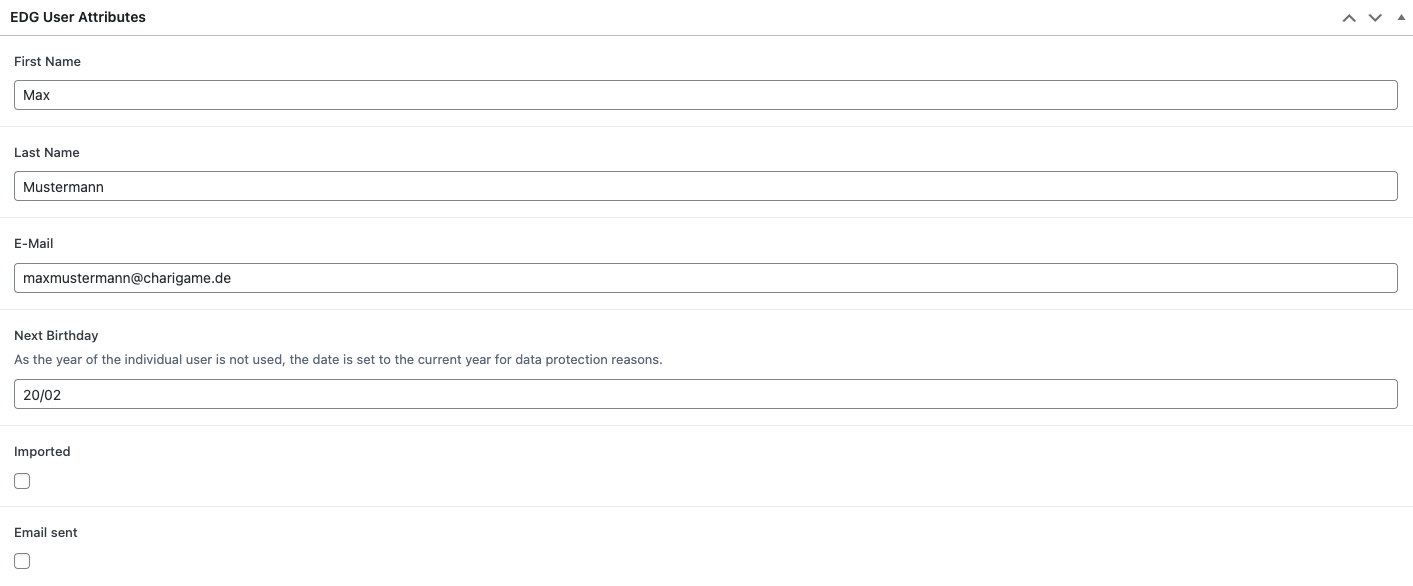
\includegraphics[width=1\textwidth]{images/legacy_users_backend}
    \caption{Users im WordPress Backend (eigene Darstellung)}
    \label{fig:users-backend-legacy}
\end{figure}

Der Bereich der Pipedrive Integration bietet die Möglichkeit Nutzer direkt über die API des \gls{crm} Systems Pipedrive zu beziehen.
Diese Funktion wurde spezifisch für ein Kundenprojekt entwickelt und bietet deshalb eine angepasst und keine universelle Funktionalität.
Die Darstellung im Backend der Piperdrive Integration zeigt Abbildung~\ref{fig:pipedrive-backend-legacy}

\begin{figure}[H]
    \centering
    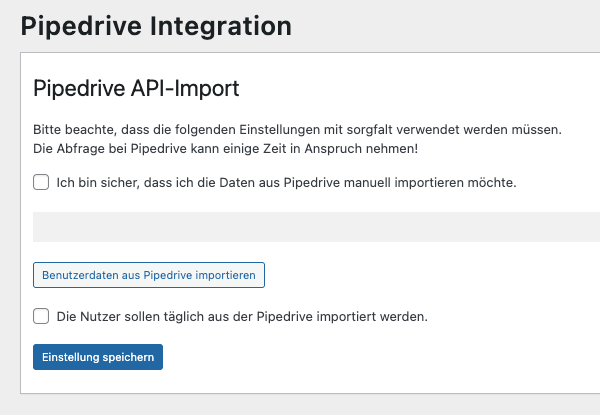
\includegraphics[width=0.5\textwidth]{images/legacy_pipedrive_backend}
    \caption{Pipedrive im WordPress Backend (eigene Darstellung)}
    \label{fig:pipedrive-backend-legacy}
\end{figure}

\\\\
\textbf{E-Mail-Settings}\\\\
Das Plugin erlaubt es, anstelle des standardmäßigen WordPress-Mailers einen eigenen \gls{smtp}-Server einzubinden.
Dafür stehen folgende Eingabefelder bereit:
\begin{itemize}
    \item SMTP-Host
    \item SMTP-Port
    \item Benutzername
    \item Passwort
    \item Verschlüsselung (\gls{tls} oder \gls{ssl})
    \item Absender-E-Mail
    \item Absender-Name
\end{itemize}
Aus Sicherheitsgründen kann das Passwort optional in der wp-config.php als Konstante \glqq CHARIGAME\_WPMS\_SMTP\_PASS\grqq{} hinterlegt werden, sodass es nicht in der Datenbank gespeichert wird.
Zusätzlich bietet die Oberfläche eine Funktion zum Versand einer Testmail, mit der sich die Konfiguration überprüfen lässt. Die Eingabemaske, befüllt mit Beispielwerten, ist in Abbildung~\ref{fig:email-backend-legacy} ersichtlich.
\begin{figure}[H]
    \centering
    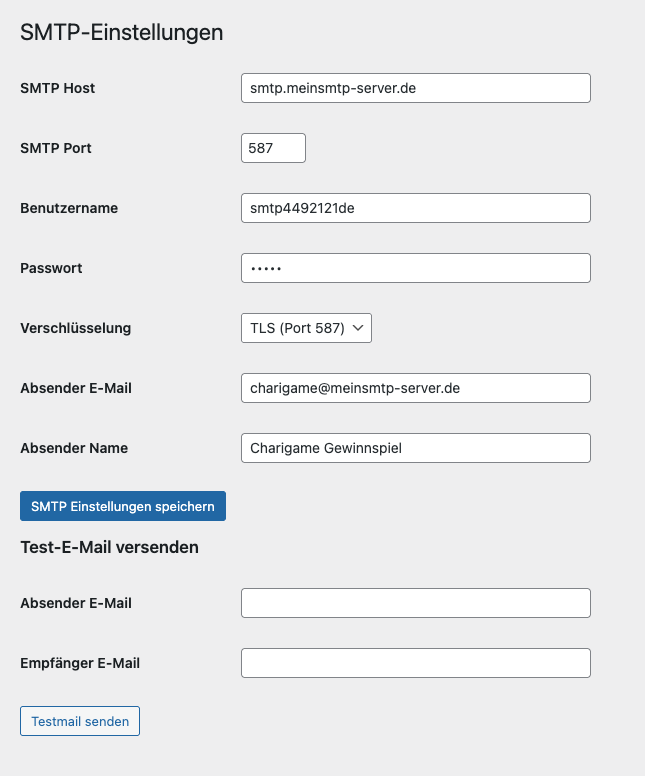
\includegraphics[width=0.7\textwidth]{images/legacy_email_backend}
    \caption{E-Mail Settings im WordPress Backend (eigene Darstellung)}
    \label{fig:email-backend-legacy}
\end{figure}

Darüber hinaus bietet der Backend-View der E-Mail-Settings eine Funktion, eine Testmail an eine ausgewählte Adresse zu senden, um die Einstellungen auf Ihre Richtigkeit prüfen zu können.

\\\\
\textbf{Data Table}\\\\
Die Data Table dient als zentrales Dashboard, um die Ergebnisse und Kennzahlen der Spendenkampagnen auf einen Blick darzustellen.
Angezeigt werden u. a.:
\begin{itemize}
    \item erstellte Kampagnen
    \item zugehörige Spendenempfänger
    \item Benutzername
    \item aktueller Spendenstand (in Euro)
    \item Nutzerübersicht mit einzigartigen Game Codes
\end{itemize}
Darüber hinaus werden weitere Metriken bereitgestellt, darunter Valid From, Valid Until, Last Played, Highscore, Recipient 1–3 sowie E-Mail sent, wie in Abbildung~\ref{fig:datatable-backend-legacy} zu sehen ist.
Die genaue Bedeutung dieser Kennzahlen ist in Tabelle~\ref{tab:metriken_datatable} im Anhang erläutert.

\begin{figure}[H]
    \centering
    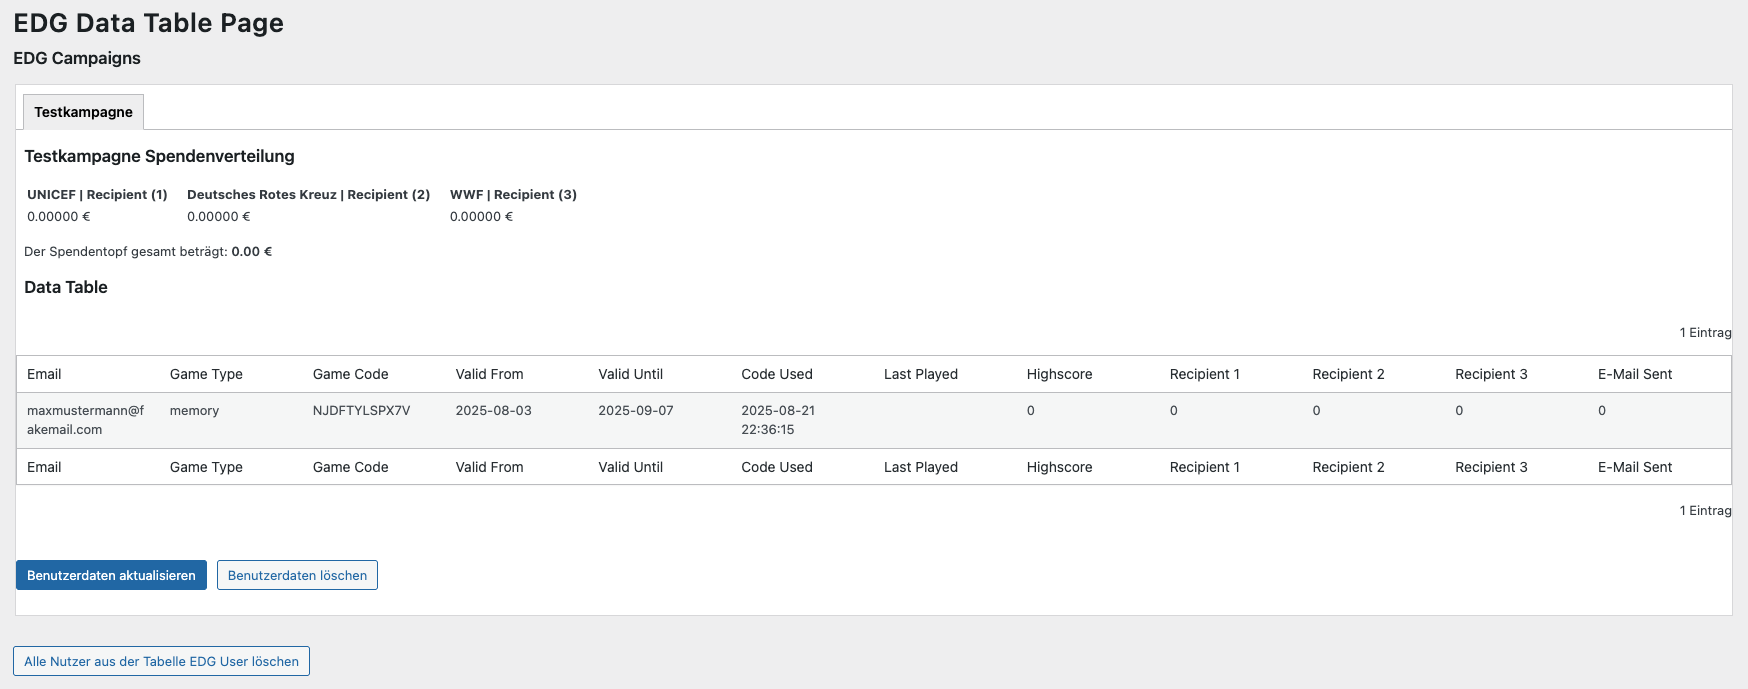
\includegraphics[width=1\textwidth]{images/legacy_datatable_backend}
    \caption{Data Table im WordPress Backend (eigene Darstellung)}
    \label{fig:datatable-backend-legacy}
\end{figure}

\newpage
\textbf{Campaigns}\\\\
Die Campaigns stellen das zentrale Element von Charigame dar und repräsentieren den konzeptionell und technisch komplexesten Bereich des Plugins.
Dieser Bereich ermöglicht deren Steuerung über eine vielzahl von Konfigurationsmöglichkeiten.
Der gesamte Ablauf einer Kampagne kann innerhalb des WordPress-Backends abgebildet werden.
Dies umfasst sowohl die Auswahl von Spieleinstellungen als auch die Kommunikation mit den Teilnehmenden.
\\
Zu den wesentlichen Komponenten der Campaings gehören:

\begin{itemize}
\item \textbf{Allgemeine Kampagneninformationen} \\
Jede Kampagne erhält einen Titel, eine kurze Bezeichnung sowie eine ausführliche Beschreibung.
Diese Inhalte bilden die Grundlage für die Frontend-Darstellung und dienen der inhaltlichen Darstellung im oberen Bereich der Landingpage.
Zusätzliche Medien wie Logos oder Illustrationen können hochgeladen und der Kampagne zugeordnet werden.

\item \textbf{Spielmechanik} \\
Der gewünschte Spieltyp wird aus den im System verfügbaren Game Types ausgewählt.

\item \textbf{Spendenempfänger} \\
Jede Kampagne referenziert mindestens drei zuvor definierte Donation Recipients.
Diese Empfänger werden im Spiel zur Auswahl gestellt, um den erspielten Beitrag unter diesen zu verteilen.

\item \textbf{Punkte- und Spendenlogik} \\
Durch eine Highscore-Logik wird festgelegt, wie viele Punkte maximal erreichbar sind und welche Spendenwerte daraus resultieren.
Gewinnkategorien ermöglichen eine Staffelung nach erreichten Punktzahlen (beispielsweise ab 20 Punkten 4 Euro, ab 50 Punkten 10 Euro).
Ein übergeordnete Spendensumme, welche vom Unternehmen unabhängig der erzielten Spenden durch die Teilnehmer erfolgt, kann ebenfalls definiert werden.

\item \textbf{Zeitliche Steuerung} \\
In der Kampagne kann zwischen zwei Methoden der Versendung gewählt werden.
Entweder zum Geburtstag der jeweiligen Teilnehmer oder zu einem ausgewählten Datum.
Darüber hinaus lässt die Uhrzeit wählen, wann die E-Mail versendet werden soll.
Ferner lässt sich die Gültigkeit der Spielcodes definieren, die angibt wie lange sich der Teilnehmer mit seinem Code einloggen kann.
Aus den getroffenen Einstellungen resultiert dann auch das Enddatum der Kampagne.
Start- und Enddatum bestimmen diesen Gültigkeitszeitraum.

\item \textbf{Kommunikation} \\
Für jede Kampagne können individuelle E-Mail-Texte konfiguriert werden.
Diese umfassen Betreffzeile, Header, Haupttext sowie eine Signatur.
Die eingestellten Inhalte werden dann in der E-Mail genutzt, die die Nutzer über ihre Teilnahme informieren.
Optional können Social-Media-Kanäle angegeben werden, welche dann in der Mail angezeigt werden.

\item \textbf{Call-to-Action} \\
Abschließend lassen sich Call-to-Action Bereiche aufbauen. Hierzu werden Headline, Beschreibungstext, Button-Beschriftung und Ziel-URL definiert.
Der \gls{cta} motiviert Teilnehmende nach Abschluss des Spiels zu weiteren Aktionen, beispielsweise dem Besuch einer Unternehmensseite.
\end{itemize}

Im Anhang der Arbeit ist die gesamte Landingpage (vgl. Abbildung~\ref{fig:landing-frontend-legacy}), die Seite der Spendenverteilung (vgl. Abbildung~\ref{fig:distribution-frontend-legacy}) und die Dankesseite (vgl. Abbildung~\ref{fig:dankesseite-frontend-legacy}) dargestellt.

\subsection{Verwendete Technologien}
Für die Umsetzung der Charigame-Einstellungen im Frontend und Backend kam eine Vielzahl an Technologien zum Einsatz.
Im Folgenden werden diese näher vorgestellt und in ihrem technischen Kontext erläutert.

\begin{itemize}
    \item \textbf{WordPress Plugin-Stack}\\
    Die Kernfunktionalität basiert auf WordPress-APIs.
    Eingesetzt wurden u. a. \gls{wp} List Table für die Darstellung von Tabellen im Admin-Dashboard, die Enqueue-Mechanismen von WordPress zum Einbinden von Skripten und Styles, sowie AJAX-Hooks für asynchrone Requests.\\
    Zusätzlich werden Register Activation Hooks und Template Include genutzt, um das Plugin beim Aktivieren einzubinden und die Views zu steuern.\\
    jQuery wird aus einem \gls{cdn} eingebunden und dient an einigen Stellen als Hilfsbibliothek für Interaktionen.\\
    Für den E-Mail-Versand und Tests kommt PHPMailer über die WordPress-Funktion wp\_mail zum Einsatz.\\
    Mit Advanced Custom Fields (ACF/ACF Pro) werden zusätzliche Metadaten für Inhalte verwaltet, die über die funktionen get\_field() intensiv genutzt werden.\\
    Außerdem wurden WP Cron Jobs bzw. Scheduled Tasks vorbereitet, um zeitgesteuerte Abläufe im Plugin zu ermöglichen.

    \item \textbf{Frontend und JavaScript}\\
    Für Animationen wird die \gls{GSAP} 3 eingesetzt.
    Neben der Kernbibliothek sind auch Plugins von GSAP wie Observer, ScrollTrigger, MotionPathPlugin und Draggable integriert, die komplexe Animationen und Interaktionen ermöglichen.\\
    Visuell wird ebenfalls Confetti \gls{js} für animierte Partikeleffekte eingesetzt.\\
    Für das Tower-Spiel wird Three.js genutzt, eine leistungsfähige 3D-Bibliothek, die sowohl lokal eingebunden als auch als \gls{npm}-Abhängigkeit installiert ist.\\
    Darüber hinaus existiert ein eigenes kleines Spiele-Framework im Ordner „games“, das z. B. Memory- und Tower-Spiele enthält und durch eigene Hilfsskripte wie helper.js und picker.js ergänzt wird.

    \item \textbf{CSS und Build-Prozess}\\
    Das Styling basiert auf Tailwind CSS, das über einen \gls{cli}-Buildprozess in Kombination mit npm-Skripten (build:css, watch:css) verarbeitet wird.
    Zusätzlich werden dynamische Theme-Farben generiert, die in einer tailwind-colors.css gespeichert und über eine PHP-Funktion automatisch aktualisiert werden.

    \item \textbf{Package- und Task-Runner}\\
    npm dient als zentraler Package Manager für JavaScript-Bibliotheken und Build-Skripte.
    Ergänzend kommt Grunt als Task-Runner zum Einsatz, unter anderem für Internationalisierung (grunt-wp-i18n) und die automatisierte Erstellung von Readme-Dateien (grunt-wp-readme-to-markdown).
    Grunt selbst wurde in der praktischen Anwendung jedoch nie wirklich verwendet.

    \item \textbf{Weitere Aspekte}\\
    Neben den genannten Technologien werden AJAX-APIs für die Kommunikation zwischen Frontend und Backend genutzt, beispielsweise um aktuelle Spendenbeträge dynamisch abzufragen.\\
    Custom Post Types und Admin-Menüs erweitern die Standardfunktionalität von WordPress, sodass eigene Inhalte und Einstellungen im Backend verwaltet werden können.
\end{itemize}
\subsection{Architektur}

Die Architektur des Plugins ist insgesamt einfach gehalten und stark auf eine zentrale Datei ausgerichtet. Sämtliche Kernfunktionen laufen in der Hauptdatei elancer-donate-games-plugin.php zusammen, die Custom Post Types, Admin-Menüs, Datenbankoperationen, AJAX-Endpunkte, Template-Overrides sowie das Enqueueing von Skripten und Styles koordiniert. Der Code ist überwiegend prozedural, enthält aber einzelne objektorientierte Elemente (z. B. in den Klassen EDGAddons oder EDG Data Table), die alle im Namespace \emph{elancer} organisiert sind.

\begin{itemize}
    \item \textbf{Backend}\\
    Im Backend werden Menüs und Tabellenansichten sowie eine SMTP-Konfigurationsseite bereitgestellt. Das Dashboard ist jedoch sehr rudimentär: Es zeigt lediglich Rohdaten in Tabellenform, bietet aber weder aussagekräftige KPIs noch visuelle Darstellungen oder interaktive Analysefunktionen.

    \item \textbf{Frontend}\\
    Das Frontend umfasst die Einbindung von Tailwind CSS, die Spiele-Module sowie externe Bibliotheken wie GSAP und Three.js. Über Template-Overrides werden eigene Views in WordPress eingebracht, was eine gewisse Anpassung erlaubt. Die Gestaltung bleibt insgesamt funktional, aber ohne ausgeprägtes visuelles Design.

    \item \textbf{Datenzugriff}\\
    Der Datenzugriff erfolgt direkt über die WordPress-Datenbankschnittstelle \emph{wpdb}. Eine eigene Tabelle (wp\_edg\_game\_data) wird per dbDelta angelegt, ohne zusätzliche Abstraktionsschicht oder \gls{orm}. Inhalte und Konfigurationen basieren stark auf ACF Pro, das an vielen Stellen über get\_field() aufgerufen wird. Dynamische Farben werden über eine in PHP generierte CSS-Datei (tailwind-colors.css) eingebunden.

    \item \textbf{Build- und Tooling-Umfeld}\\
    Für den Build-Prozess kommt ein Tailwind-CLI-Workflow zum Einsatz, gesteuert über npm-Skripte. Grunt unterstützt Aufgaben wie Internationalisierung und die Generierung von Readme-Dateien. Composer, PHP CodeSniffer (inklusive WPCS und PHPCompatibility) sowie PHPUnit sorgen für Codequalität. Ergänzend prüft eine CircleCI-Pipeline die Kompatibilität des Plugins mit verschiedenen PHP-Versionen.

    \item \textbf{Einschränkungen und Schwächen}\\
    Die Bearbeitung von Landingpages ist nur eingeschränkt möglich, viele Texte sind fest im Code hinterlegt und bieten damit wenig Flexibilität. Das Dashboard liefert nur eine einfache Datenübersicht und bleibt visuell schlicht. Sicherheitsaspekte wurden nur teilweise berücksichtigt: Manche AJAX-Endpunkte verzichten auf Nonce- oder Berechtigungsprüfungen, und an einigen Stellen fehlt sauberes Escaping. Auch die Datenbank-Constraints sind uneinheitlich, wodurch doppelte Spielcodes möglich sind. Darüber hinaus erschwert die starke Bündelung der Logik in einer Datei die Wartbarkeit. Designprinzipien wie Service- oder Repository-Muster sind nicht umgesetzt, und auch die Einbindung von Assets ist wenig optimiert, da Skripte und Bibliotheken ohne Bündelung oder Minifizierung geladen werden.
\end{itemize}
\vspace{0.5em}
Insgesamt ergibt sich damit ein pragmatisches Architekturkonzept, das die Umsetzung beschleunigt hat, jedoch klare Grenzen in Bezug auf Flexibilität, Wartbarkeit und Sicherheit erkennen lässt.

\section{Stakeholder und Nutzungskontext}
Als Stakeholder wurden seitens der elancer-team GmbH die folgenden Gruppen identifiziert:
Viereck mit den Stakeholdern.

Nutzungskontext: Für

CPTs nice
Screenshots Frontend Backend zeigen
\section{Gesetzte Anforderungen an die Weiterentwicklung}

Für den zu bearbeitenden Part im Kaptiel 4 sind Praxispart mindestens die folgenden Anforderungen gesetzt:
\subsection{Technische Anforderungen}
\begin{itemize}
    \item Das System muss die Abhängigkeit von der PRO-Version des Plugins ACF (Advanced Custom Fields) entfernen.
    \item Das System muss gängige WordPress-Plugin-Best-Practices befolgen.
    \item Das System soll gängige Security-Best-Practices der WordPress-Developer-Ressourcen berücksichtigen.
\end{itemize}



\subsection{Funktionale Anforderungen}
\begin{itemize}
    \item Das System muss die Landingpage mit dem Gutenberg-Editor editierbar machen.
    \item Das System muss Gutenberg-Blöcke bereitstellen, die die bestehende Landingpage abbilden können.
    \item Das System soll eine verbesserte Version des Dashboards bereitstellen.
    \item Das System soll eine bessere Übersicht für Nutzer bieten.
    \item Das System soll eine verbesserte Möglichkeit bieten, Inhalte zu bearbeiten.
\end{itemize}

\section{Abgrenzung des Projektumfangs}
Zur Abgrenzung des Projektumfangs wurden jetzt hier die Anforderungen aufgebaut.
Ferner gilt es begleitend die schriftliche Ausarbetiung auszuführen.
Damit ein wissenschaftlicher konsens gefunden werden kann muss das ergebnis am ende evaluiert werden und das ergebnis kritisch betrachtet werden.
Ferner soll der weitere horizont für das zukünfitge vorgehen festgelegt werden und mögliche erweiterungen oder anpassungen angesprochen werden.
